\subsection*{Example 1}

\begin{itemize}
	\item 2 rovers, 4 waypoints, 2 objectives
	\item $energy(R_0) = 21$
	\item $energy(R_1) = 24$
	\item $C_0$ : $R_0$ LR
	\item $C_1$ : $R_1$ LR
\end{itemize}

\subsubsection*{Original Goals \& Properties}
\begin{minipage}[t]{0.45\textwidth}
	\begin{itemize}
		\item SD $WP_0$
		\item SD $WP_1$
		\item RD $WP_0$
		\item RD $WP_1$
		\item I $O_1$ LR
	\end{itemize}
\end{minipage}
\begin{minipage}[t]{0.45\textwidth}
	\begin{itemize}
		\item $i(O_1, C_0)$
		\item $i(O_1, C_1)$
		\item $i(O_1, WP_0)$
		\item $sr(O_1, WP0)$
	\end{itemize}
\end{minipage}

\begin{center}
\scriptsize
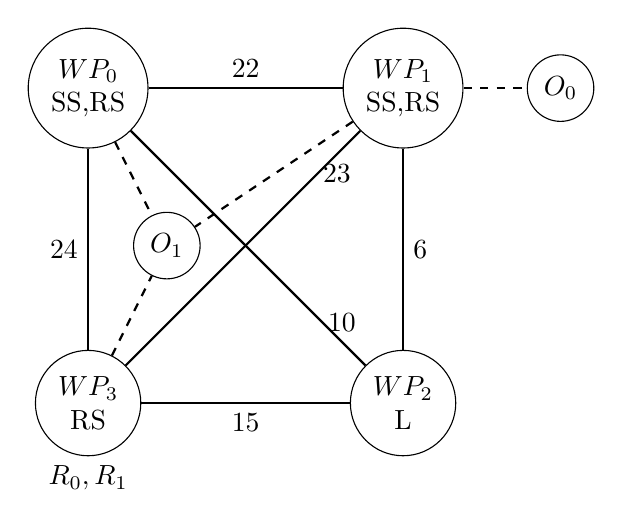
\begin{tikzpicture}
	\node[draw, circle, align=center,
		] (l0) at (0,0) {$WP_0$\\ SS,RS};
	\node[draw, circle, align=center,
		] (l1) at (4,0) {$WP_1$\\ SS,RS};
	\node[draw, circle, align=center,
		] (l2) at (4,-4) {$WP_2$\\ L};
	\node[draw, circle, align=center,
			label=below:{$R_0,R_1$},
		] (l3) at (0,-4) {$WP_3$\\ RS};


	\node[draw, circle, align=center] (o0) at (6,0) {$O_0$};
	\node[draw, circle, align=center] (o1) at (1,-2) {$O_1$};

	\draw[thick] (l0) to node[above] {22} (l1);
	\draw[thick] (l1) to node[right] {6} (l2);
	\draw[thick] (l1) to node[below, pos=0.1] {23} (l3);
	\draw[thick] (l0) to node[left] {24} (l3);
	\draw[thick] (l2) to node[below] {15} (l3);
	\draw[thick] (l0) to node[above, pos=0.9] {10} (l2);


	\draw[thick, dashed] (l0) to (o1);
	\draw[thick, dashed] (l1) to (o1);
	\draw[thick, dashed] (l3) to (o1);
	\draw[thick, dashed] (l1) to (o0);
\end{tikzpicture}
\end{center}



\begin{figure}[ht]
\begin{center}
	\includegraphics[scale=0.4]{data/graph_rovers_p02.pdf}
\end{center}
\caption{plan-property dependency graph (PDG) example 01}
\end{figure}


\subsubsection*{Goal-Fact Dependencies}
\begin{itemize}
	\item $i(O_1,WP_1),sr(O_1,WP_1)$
	\item $i(O_1,WP_1),i(O_1,WP_3)$
	\item $i(O_1,WP_0),i(O_1,WP_3)$
	\item $i(O_1,WP_0),i(O_1,WP_1)$
	\item $i(O_1,R_0),sr(O_1,WP_1)$
	\item $i(O_1,R_0),i(O_1,WP_0)$
	\item $i(O_1,R_0),i(O_1,R_1)$
	\item $i(O_1,C_1),i(O_1,R_0)$
	\item $i(O_1,C_0),sr(O_1,WP_1)$
	\item $i(O_1,C_0),i(O_1,WP_0)$
	\item $i(O_1,C_0),i(O_1,R_1)$
	\item $i(O_1,C_0),i(O_1,C_1)$
	\item $crd(WP_0),i(O_1,R_1),i(O_1,WP_1)$
	\item $crd(WP_0),i(O_1,C_1),i(O_1,WP_1)$
	\item $csd(WP_0),i(O_1,R_1),i(O_1,WP_1)$
	\item $csd(WP_0),i(O_1,C_1),i(O_1,WP_1)$
\end{itemize}





\subsection*{Example 2}

\begin{itemize}
	\item 2 rovers, 5 waypoints, 2 objectives
	\item $energy(R_0) = 4$
	\item $energy(R_1) = 3$
	\item $C_0$ : $R_0$ C, HR, LR
	\item $C_1$ : $R_0$ C, LR
	\item $C_2$ : $R_1$ C, HR, LR
	\item $C_3$ : $R_1$ C, LR
\end{itemize}

\subsubsection*{Original Goals \& Properties}
\begin{minipage}[t]{0.45\textwidth}
	Goals
	\begin{itemize}
		\item SD $WP_1$
		\item SD $WP_3$
		\item RD $WP_1$
		\item RD $WP_3$
		\item I $O_1$ LR
		\item I $O_1$ C
	\end{itemize}
\end{minipage}
\begin{minipage}[t]{0.45\textwidth}
	Properties
	\begin{itemize}
		\item $i(O_1, C_0)$
		\item $i(O_1, C_1)$
		\item $i(O_1, C_2)$
		\item $i(O_1, C_3)$
		\item $i(O_1, R_0)$
		\item $i(O_1, R_1)$
		\item $i(O_1, WP_4)$
		\item $sr(O_1, WP2)$
	\end{itemize}
\end{minipage}


\begin{center}
\scriptsize
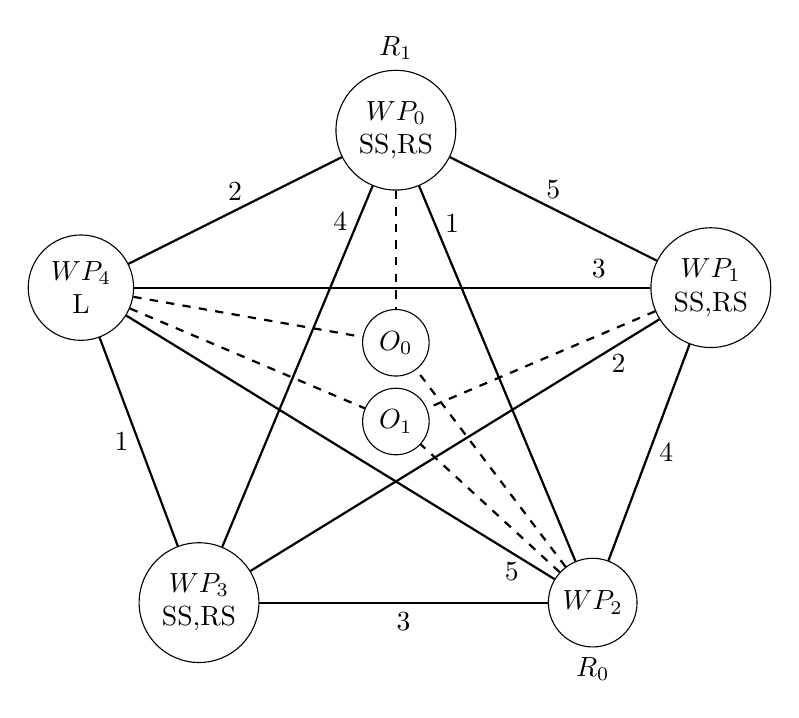
\begin{tikzpicture}
	\node[draw, circle, align=center,
			label=above:{$R_1$},
		] (l0) at (0,0) {$WP_0$\\ SS,RS};
	\node[draw, circle, align=center,
		] (l1) at (4,-2) {$WP_1$\\ SS,RS};
	\node[draw, circle, align=center,
			label=below:{$R_0$},
		] (l2) at (2.5,-6) {$WP_2$};
	\node[draw, circle, align=center,
		] (l3) at (-2.5,-6) {$WP_3$\\ SS,RS};
	\node[draw, circle, align=center,
		] (l4) at (-4,-2) {$WP_4$\\ L};


	\node[draw, circle, align=center] (o0) at (0,-2.7) {$O_0$};
	\node[draw, circle, align=center] (o1) at (0,-3.7) {$O_1$};

	\draw[thick] (l0) to node[above] {5} (l1);
	\draw[thick] (l0) to node[right, pos=0.1] {1} (l2);
	\draw[thick] (l0) to node[left, pos=0.1] {4} (l3);
	\draw[thick] (l0) to node[above] {2} (l4);
	\draw[thick] (l1) to node[right] {4} (l2);
	\draw[thick] (l1) to node[below, pos=0.1] {2} (l3);
	\draw[thick] (l1) to node[above, pos=0.1] {3} (l4);
	\draw[thick] (l2) to node[below] {3} (l3);
	\draw[thick] (l2) to node[below, pos=0.1] {5} (l4);
	\draw[thick] (l3) to node[left] {1} (l4);
	%\draw[thick] (l1) to node[below, pos=0.1] {23} (l3);


	\draw[thick, dashed] (l0) to (o0);
	\draw[thick, dashed] (l2) to (o0);
	\draw[thick, dashed] (l4) to (o0);
	\draw[thick, dashed] (l1) to (o1);
	\draw[thick, dashed] (l2) to (o1);
	\draw[thick, dashed] (l4) to (o1);
\end{tikzpicture}
\end{center}



\begin{figure}[ht]
\begin{center}
	\includegraphics[scale=0.4]{data/graph_rovers_p03.pdf}
\end{center}
\caption{plan-property dependency graph (PDG) example 02}
\end{figure}


\subsubsection*{Goal-Fact Dependencies}
	\textcolor{red}{TODO}

	As 6 original goals and 4 properties are too many facts to check at once only 2 properties 
	are added at once.

	\begin{enumerate}
		\item $i(O_1, C_0)$, $i(O_1, C_2)$ t=1100 sec
		\begin{itemize}
			\item $i(O_1, C_0)$, $i(O_1, C_2)$
		\end{itemize}
			They contradict by definition, but the result shows us that there exist 
			solution for both cameras.
		\item $i(O_1, C_0)$, $i(O_1, WP_4)$ t=840 sec
		\begin{itemize}
			\item $CRD(WP_1), i(O_1, C_0), i(O_1, WP_4)$
			\item $CSD(WP_1), i(O_1, C_0), i(O_1, WP_4)$
		\end{itemize}
			
		\item $i(O_1, C_2)$, $i(O_1, WP_4)$ t=10 sec\\
			nothing
		\item $ra(WP_1, R_1)$ t=525 sec
			\begin{itemize}
				\item $ra(WP_1, R_1)$ ($\rightarrow$ Question: Can rover 1 reach waypoint 1?)
			\end{itemize}
		\item $at(R_1, WP_1)$ t=7 sec
			\begin{itemize}
				\item $at(R_1, WP_1)$ $\rightarrow$ Rover 1 can not reach waypoint 1.
			\end{itemize}
	\end{enumerate}



